\documentclass{article}%

\usepackage{amsmath,amssymb,amsfonts,epsfig,amsfonts}
\usepackage{cite}
\usepackage{graphicx}
\usepackage{subfigure}
\usepackage{mathrsfs}
\usepackage{extarrows}  %
\usepackage{hyperref}
\usepackage{comment}  %
\usepackage{pgfplots} %
\makeatletter

\baselineskip=40pt
\textheight 22.5truecm
\topmargin -0.5125truein
\textwidth 15.74truecm
\oddsidemargin -0.06truein
\evensidemargin -0.06truein
\parskip=0.1in
\renewcommand{\baselinestretch}{1.2}   %

\title{ \bf Are local-mins Rare?
 \footnote{This is an informal note. }
} \vskip 1cm
\author{ Thomas Jefferson
}
\date{}

\begin{document}
\maketitle

\begin{abstract}

Analyze nonconvex optimization from topology. 

\end{abstract}

\thispagestyle{empty}




\section{Test Section}




\iffalse 
 This is commented by iffalse command, not comment.
 Not easy to be eliminated by this cleaning file. 
 \fi 

This is a percent \%.  Should stay here after running the cleaning file. 

We add a figure for testing. 

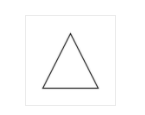
\includegraphics{images/im1_included.png}

If the code is correct, then the following figure should not appear in the cleaned tex file (
if the code is wrong in the sense that it only removes $\%$ but not the commands
after it, then the non-included figure would appear in the cleaned tex  file).


We can also check inputting other Latex Files.
This is a file in a sub-folder ``figures'', and we are supposed to see
one figure, but not two figures. 




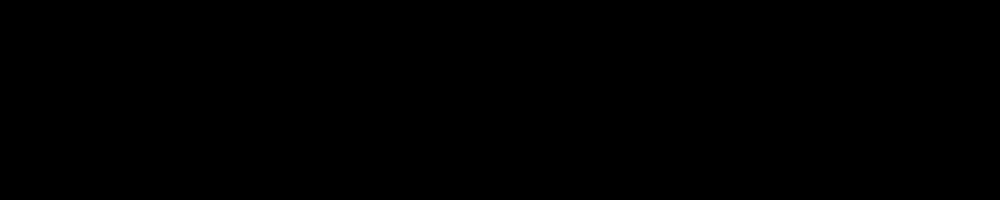
\includegraphics{images/im2_included.jpg}

% \addplot{figures/data_included.txt}




\section{Model}

This part is a test that the standard math formulas will not be affected after
running the cleaning file. 

Definition (LSC property): $\forall \bar{\alpha} \in G, \bar{x} \in L_f(\bar{\alpha}) \triangleq \{ x: f(x) \leq \bar{\alpha} \}$,
and $\forall$ sequence $\{ \alpha_i \} \rightarrow \bar{\alpha}$, we have 
$$
\exists x^i \in L_f(\alpha_i), \text{s.t. } \{ x^i\} \rightarrow \bar{x}. 
$$

Definition (GC property): For any two points $ f(\tilde{x}) < f(\bar{x}) $, there exists a sequence $ \{x^i\} \in C$ converging to $ \bar{x} $
such that 
\begin{equation}
f(x^i)\leq \frac{1}{i} f(\tilde{x}) + (1 - \frac{1}{i})f(\bar{x}). 
\end{equation} 


 \vspace{0.3cm}

{\footnotesize
\bibliography{refs}
}


\end{document}



